It is not only for stack and heap elements that we need to store type
information. Sub-routines and field definitions also have type information which
we need to keep track of, but the information does not necessarily describe the
same things. For instance, a stack or heap element has types describing the type
of its value. A sub-routine will need have a type signature, describing the
types of it's parameters, a name and possible properties. Similarly a field
definition will also have a name and other possible properties. In the eyes of
the machine, all of these are regarded as types describing some internal
structures.

Therefore, we need to abstract the way we store type information a level higher,
letting us better describe different kinds of types, be it a sub-routine, field
definition or a regular type from the type table discussed in earlier in
Section~\ref{sec:design:types}. Instead of storing the different kinds of
information in different locations, there is a centralized table, containing
all, what we call, meta information. This is named the metadata table and will
need to be dynamically sized to support reflection and generation of new types
at run-time.

All metadata objects in the machine have a tag defining which type of
information it contains.

\begin{ccode}
enum meta_tag_e {
    TYPE,
    FIELD_DEF,
    SUBROUTINE_DEF,
    SUBROUTINE_REF
};
typedef enum meta_tag_e meta_tag;

struct meta_base_s {
    meta_tag tag;  ///< Kind of meta
    uint32_t hash; ///< Unique hash for lookup
};
typedef struct meta_base_s meta;

/** \brief meta describing a type */
struct meta_type_s {
    meta base;

    type *type;
};
typedef struct meta_type_s meta_type;
\end{ccode}

Using this method of ``inheriting'' structs, a type pointer can be cast to the
correct struct type based on the value of its \code{tag} field.

We will describe each type of metadata information in turn.

\subsubsection{Types}
\label{sec:implementation:meta:types}

The executable file that contains the program to be run, defines a type table
for the types created needed during run-time. Throughout the executable, these
types are referenced by the type's index in this table. This table is static, so
the machine can analyze how many types it contains. The types will be parsed
from the executable and added to the global metadata table lazily. This reduces
the initial overhead of parsing the executable and avoids loading types that
will not be used during run-time.

The machine's built-in types are described by a type tag, implemented as an enum
in the same way as the \code{meta\_tag}. The enum's integer value is used to
describe its index in the metadata table, and there will always only be a single
instance of each type, so two equal types can never be referenced by two
different pointers, similar to how DWARF types are stored (as described in
Section~\ref{sec:design:types:dwarf}). This lets the machine check type equality
simply by comparing the type pointers.

All types in the machine are stored internally through structs. Simple types are
represented by the {\tt type\_base} struct, which is extended in compound
types.

Types are passed around in the machine by the {\tt type} name. If the type is
for instance a reference, i.e.~implementing the {\tt type\_ref}, it is cast so
its reference specific attributes can be accessed. The type of a type is checked
through the tag, defined in {\tt type\_base}. Another important entry in the
type structure is the size attribute. This is essential, as it tells the machine
how much memory is needed to store a value of that type on either the stack or
heap. The exception is Composite types whose size is computed during run-time
because it is not part of the type definition per s\'e.

Types from the executable are mapped from its index in the binary type table to
the machine's metadata table. As the ELF meta table is of static size, this will
be a simple integer array, mapping binary metadata indices to the machine's
internal metadata entries in the metadata table. The metadata entries will be
parsed lazily, i.e.~the first time the program tries to look up a metadata entry
through its index in the ELF metadata table.

The machines internal metadata table is implemented through a hash map, where
each meta entry can be looked up through it's hashed value. Having implemented
the metadata table as a hash table lets us look up entries in constant time,
avoiding the overhead of iterating. The only requirement of the hashing function
is that it makes unique hashes for metadata entries that are equal. This is
currently done with a simple implementation of Bob Jenkins' One-at-a-time
hash\cite{jenkins}. We have chosen this hash function due to relatively good
speed and uniqueness, compared to more complex hashing functions. Bob Jenkins
himself has written article comparing several similar functions and their
running speed, which we used as reference\cite{jenkins}. To get a reference to a
built-in type, one can look it up through a look-up function, which takes a
metadata hash. This can be done through a strict function which thrown an
exception if the hash is not found, or a lazy function which will generate the
new meta entry if not found. This is especially useful for looking up types that
are not guaranteed to already be found in the metadata table, such as reference
types used when boxing (see Section~\ref{NEEDED}).

% TODO how to structure this?

\subsubsection{Composite Types}

Composite types are used to describe heap objects, stack objects and
scopes. They consist of a name and a set of members which are implemented as an
array of pointers to metadata entries which must be either fields or
sub-routines. Members are looked up during run-time by use of a metadata entry
that describes the field or sub-routine. The idea is that a heap object's (or
stack object's or scope's) associated type includes its members, so modification
of the heap object's actual data is possible by providing the definition of the
desired member that maps to a field or sub-routine. See
Section~\ref{sec:implementation:meta:fields}
and~\ref{sec:implementation:meta:sub-routines} for details of how fields and
sub-routines are used to modify a heap object.

The list of members is dynamic meaning that members can be added or removed
during run-time. This is a useful feature for dynamic languages in which it is a
common feature to be able to modify the list of properties on an object during
run-time. The current implementation however does not support this, but would
likely be implemented via run-time library functions.

Composite types also include a list of properties that defines certain aspects
of its behavior. These are not current implemented, but one such property is
{\em strict layout}, which tells the machine that the members of an object
instantiated with the composite type must be laid out in memory in the order
which they are defined. This can be useful for compilers that run unsafe code to
manually get and set data on members.

\subsubsection{Floating-Point Value Types}

When handling floating-point precision numbers we will, as aforementioned, use
the IEEE 754 standard\cite{ieee754}. This is a technical standard defining the
arithmetic format, i.e.~the finite range and special values, rounding rules,
operations, exception handling and interchange formats. Its values include
finite numbers (within a certain maximum and minimum, depending on the size),
two infinities (positive and negative) and a NaN (not a number).

A floating-point number is represented by a sign, a fraction (also called
significant or mantissa) and an exponent. A value can have multiple alternative
representations, for instance $1.10 \cdot 10^2$ can also be written as
$11.00 \cdot 10^1$. This though, should not have any effect on the result of
arithmetic operations. When storing the number in memory, one bit is used for
sign and the rest for exponent and fraction, depending on the size. The most
common the is single and double precision, which is respectively 4 and 8 bytes
in size. Their binary representation is called {\tt binary32} and {\tt
  binary64}.

\begin{figure}[H]
  \centering
  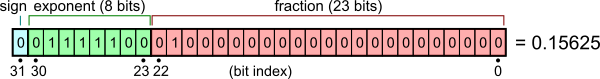
\includegraphics[scale=0.7]{images/ieee32.png}
  \caption[Caption for LOF]{IEEE-754 binary32 encoding\footnotemark}
\end{figure}
\footnotetext{IEEE-754 binary32 encoding:
  \url{https://en.wikipedia.org/wiki/Single-precision_floating-point_format}}

When parsing a {\tt binary32} we start by extracting all the relevant bits out
into separate numbers. We can then apply the following formula to get its
decimal value.

\begin{equation}
  value = (-1)^{sign} \cdot (1 + \sum^{23}_{i=1} frac_{23-i}2^{-i}) \cdot 2^{exp - 127}
\end{equation}

% type lattice

When performing arithmetic instruction on numbers, the machine enforces strong
typing and will therefore throw an exception if the operands is not of the same
type. This is to avoid common pitfalls, such as not handling overflow of
numbers, but also when doing arithmetic operations of two different types of
numbers. The compiler itself will have to truncate or convert values to matching
types before performing arithmetic operations.

Take, for instance, a program attempting to divide a floating-point precision
number by an integer number, will the result be an floating point or integer?
The only scenario where the machine itself needs to make a choice about is with
stack elements of type {\tt AnyType}. Instead of having a long list of what do
do in every case of all types, the choice will be defined by a type
lattice. This type lattice will control what type the result is of, in a given
operation between two numbers of different types.

All binary arithmetic operations follow the same type lattice. The type lattice
has the following set of rules matching which operand that is to be converted,
where the resulting conversion is also the type of the result.

\begin{itemize}
  \item If both operands is of the same type, nothing needs to be done.
  \item Otherwise, if either operand is a double floating-point precision
    number, the other operand is converted to a double also.
  \item Otherwise, if either operand is a single floating-point precision
    number, the other operand is converted to a float also.
  \item Otherwise, if either operand is of different signs, i.e. one is unsigned
    and the other is signed, the signed operand is converted to the an signed
    integer of the largest size of the two operands.
  \item Otherwise, the operands is of integer types of the same sign, where we
    return the largest of the two.
\end{itemize}

If none of the rules apply it will mean that at least one of the given operands
is of a type not supporting arithmetic operations. In this case, an exception
will be thrown.

If a type is converted to a type of smaller size, the value it truncated and has
a risk of overflowing, changing the value of the number. The {\tt noOverflow}
prefix defines if an exception should be thrown if overflow occurs.

\subsubsection{Fields}
\label{sec:implementation:meta:fields}

Fields are also a type of metadata, describing a member of a {\tt Composite}
type, in the form of field definition. It is important to note that fields are
not types themselves, like {\tt Composite} is, but a meta element describing a
field definition. Consequently, a field definition has a type element describing
the type of its content.

The internal data representation of a field definition, is as all other meta
types, an extension of the {\tt meta\_base} struct, giving it a type of meta, in
the form of a tag, and a unique hash. The field definition struct, {\tt
  meat\_field} extends this by adding a name, which is a index into the string
table, an integer offset, which is the distance where its value is stores from
the beginner of the heap object, and lastly a type describing its content. In
addition to these it a has an arbitrary number of properties and versions, which
are not implemented. The version element is to support dynamic languages
which can be extended or monkey patched, as Rubyists like to call it. Therefore,
a number of similar fields can exist in memory, which are distinguished by
version. % TODO

A field can be defined with set of properties, modifying its functionality. Such
properties are {\em abstract}, where the field is not actually initialized, only
declared. This is useful for languages with interfaces or abstract methods, akin
to Java's abstract classes and methods where another class can extend the
abstract class, implementing its already defined fields and methods.

Another property is {\em final}, where the the specific content of the field
cannot be changed. If the content is a reference, for instance, the referenced
value will always be the same, but the value of reference may still be mutated.

\subsubsection{Sub-Routines}
\label{sec:implementation:meta:sub-routines}

The last kind of metadata is a sub-routine which defines an executable set of
instructions. It is similar to a function (as in C), with the exception that a
sub-routine does not return a value. Rather, as described in
Section~\ref{sec:design:exec:sub-routine}, a sub-routine can modify values by
reference or by modifying stack elements upward into the stack, outside its own
stack frame.

A sub-routine defines a low-address which is the entry point of execution upon
invocation, and a high-address which is the the last instruction belonging to
it, together defining the address bounds of the sub-routine. Branching
instructions are not allowed to target addresses outside the bounds of the
currently executing sub-routine because it can be a security risk to execute
arbitrary code. This becomes an issue when linking multiple executables which
are ignorant of each others program data.

A special type of sub-routine is that defined by the run-time. Instead of using
a byte code address, they are currently hardcoded into the machine and are
invoked via a C function pointer. The run-time function is executed and then
execution continues as before, meaning that the semantics from the running
program's point of view are identical to that of usual sub-routines. The machine
distinguishes between run-time sub-routines and normal ones by their name;
language implementations are required to mangle the names of all symbols
(i.e.~field, sub-routines and type names) and prepend them with the ``\_''
characters. Upon invocation, if the name of the sub-routine does not start with
``\_'' then it is dispacted as a run-time function and if not the program
counter is changed to the sub-routines entry address.

The arguments that are accepted by a sub-routine are defined in its metadata
entry, but are currently not implemented. They would be used to verify that the
type of the elements currently on the stack align with the types of arguments,
and if not throw an exception.

%%% Local Variables:
%%% mode: latex
%%% TeX-master: "../report"
%%% End:
